\documentclass[prl,twocolumn,showpacs]{revtex4}

\usepackage{epsfig,color,graphicx,amsmath}
\begin{document}
\newcommand{\ltwid}{\mathrel{\raise.3ex\hbox{$<$\kern-.75em\lower1ex\hbox{$\sim$}}}}
\newcommand{\gtwid}{\mathrel{\raise.3ex\hbox{$>$\kern-.75em\lower1ex\hbox{$\sim$}}}}
\newcommand{\bra}{\langle}
\newcommand{\ket}{\rangle}
%\newcommand{\sill}{\psi_\mathrm{SILL}}
\newcommand{\sill}{\psi}
\newcommand{\trace}{{\rm Tr}}
\newcommand{\ntilde}{\tilde{n}}
\newcommand{\stilde}{\tilde{s}}
\newcommand{\atilde}{\tilde{\alpha}}
\newcommand{\new}{\color{red}}
\newcommand{\old}{\color{black}}
\newcommand{\bea}{\begin{eqnarray}}
\newcommand{\eea}{\end{eqnarray}}
\def\nn{\nonumber\\}

\bibliographystyle{apsrev}

\title{Establishing a fundamental connection between the covalent component of the
hydrogen bonding network and properties of liquid water}

\author{Yifei Shi}
\affiliation{Department of Chemistry, McGill University, 801 Sherbrooke St. West, Montreal, QC H3A 0B8, Canada}

\author{Hayden Scheiber}
\affiliation{Department of Chemistry, McGill University, 801 Sherbrooke St. West, Montreal, QC H3A 0B8, Canada}

\author{Rustam Khaliullin}
\affiliation{Department of Chemistry, McGill University, 801 Sherbrooke St. West, Montreal, QC H3A 0B8, Canada}

%\date{\today}

\begin{abstract}
Many remarkable properties of liquid water originate from the ability of water molecules to form hydrogen bond, which is a combination of electrostatic, induction, dispersion and covalent interactions. In this work, we developed an ab initio molecular dynamics method that enabled us to adjust the spatial extent of the covalent component of interactions between water molecules in simulations. We show that for room-temperature liquid water, a seemingly small amount of electron transfer has a profound effect on observable properties of liquid water. In particular, the tetrahedronal structure, O-H stretch mode and viscocity are all significantly determined by covalent interactions.


\end{abstract}
\maketitle

\section{Introduction} 

Detailed understanding of the physical nature of hydrogen bonding (HB) between molecules in water is essential to unravel origins of the unique properties of this ubiquitous and important liquid. It has been known since the dawn of quantum mechanics that hydrogen bonding is a complex phenomenon that arises from the interplay of several distinct effects: interaction between molecules’ permanent multipoles (dipoles, quadrupoles, etc.), polarization, dispersion, and donor-acceptor orbital interactions that lead to partial electron transfer between molecules. Recent developments in electronic structure methods have helped to make progress towards solving a long-standing problem of quantifying the individual contributions of these effects to the energy of hydrogen bonding. One last unresolved issue has been the extent of intermolecular charge transfer in hydrogen bonding \cite{isaacs1999covalency,ghanty2000hydrogen,stone2017natural}.
Natural bond orbital (NBO) analysis\cite{weinhold1998natural} and natural energy decomposition analysis \cite{glendening1994natural} suggest that charge transfer (CT) is predominant \cite{schenter1996natural,glendening2005natural,weinhold2005resonance} because, if charge transfer is neglected, NBO analysis shows no binding at the water-dimer equilibrium geometry. However, other earlier decomposition methods \cite{kitaura1976new,bagus1984new,bagus1992decomposition,stevens1987frozen,chen1996energy} as well as as most recently developed alternatives \cite{mo2000energy,misquitta2003dispersion,khaliullin2007unravelling} estimated that CT contributes only around 20\% of the overall binding energy. After a debate spanning several decades, it is becoming clear that NBO is not optimized to treat intermolecular interactions\cite{stone2017natural}, and covalent donor-acceptor component contributes only a small portion to the overall binding energy between water molecules in small clusters \cite{stevens1987frozen,chen1996energy,piquemal2005csov,khaliullin2009electron,cobar2012examination}.



The success of energy decomposition techniques allowed us to look beyond a simple contribution of charge transfer to the interaction energy and to establish a fundamental connection between physical components and the observed properties of water – an area, in which our knowledge remains rudimentary at best. In this work, we coupled ab initio molecular dynamics to a recently developed energy decomposition method for periodic systems \cite{Khaliullin2013JCTC} to perform an unprecedented computational study that enabled us to quantify the contribution of the covalent component of hydrogen bonding to the structural, dynamical and spectroscopic properties of liquid water at ambient conditions. We showed that even a seemingly insignificant covalent component of hydrogen bonding has a profound effect on the properties of water.


\section{Methods}

To isolate the effect of the covalent component of hydrogen bonding on the properties of liquid water, we performed ab initio molecular dynamics simulations using a special version of density functional theory based on absolutely localized molecular orbitals (ALMO)\cite{khaliullin2006efficient,Khaliullin2013JCTC}. In ALMO, each molecular orbital (MO) is expanded in terms of the atomic orbitals (AOs) of a fragment containing a certain number of molecules, thus the charge transfer between molecules can easily be adjusted by changing the number of molecules in the fragment. In this work we set the fragment to have only one molecule, totally excluding any charge transfer. 
\new{what to say about ALMO MD?} \old


In order to compare properties of liquid water with and without charge transfer, we look at the system described by ALMO with zero charge transfer, and the system described by normal DFT. The former will be refered to as localized system and the latter delocalized or reference system. We use BLYP functional, TZV2P basis set, and D3 dispersion correction for both systems. The density of these systems are set to be 1.04 g/cm$^3$ for a MD simulation with NVT ensemble at a temperature of 298K. Since properties like density or pressure can be affected by covalency, we also look at a third system whose density is determined by a NPT simulation at a constant pressure of 1atm. This system will be denoted by high density localized system.



\section{Results}

The Oxygen-Oxygen radial distribution function (RDF) is shown in Fig~\ref{Fig:RDF}. It is clear that the molecules in the localized system turns to be further away, since the interaction between molecules are weaker. 

\begin{figure}
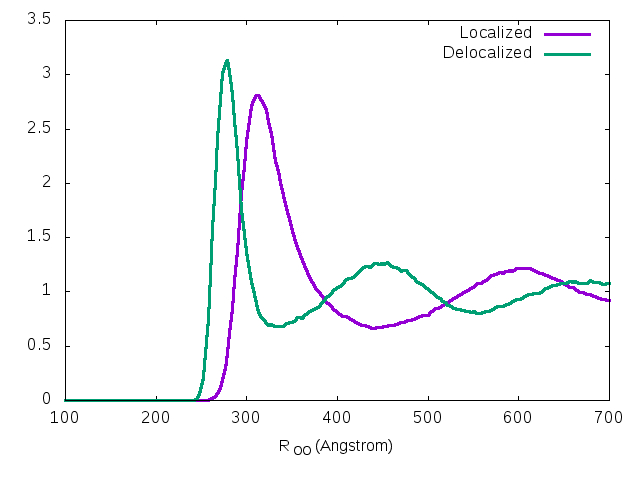
\includegraphics[width=0.4\textwidth]{RDF}
\caption{Oxygen-Oxygen radial distribution function for localized and delocalized water systems. The calculation was done for  125 water molecules with NVT ensemble. The average distance between molecules and the position of the first solvent shell are all larger for the localized system.} \label{Fig:RDF}
\end{figure}


The infared spectrum for the system is calculated using TRAVIS. Fig~\ref{Fig:IR} shows the infared(IR) spectrum of the localized and reference systems. For comparison, the IR spectrum of none-interaction water vapor is also shown. The O-H stretch modes of the localized system do not show the broadening and shift due to HBs, as in the delocalized system. Which implies that these modes are very sensitive to covanlency, and without covanlecy, they are very similar to that of the none-interacting molecules. Another difference between the localized and delocalized system is the intermolecular modes, they are shifted to lower energy because the intermolecular bonding in localized system is weaker. The bending modes remain roughly the same for localized, delocalized and vapor systems.

\begin{figure}
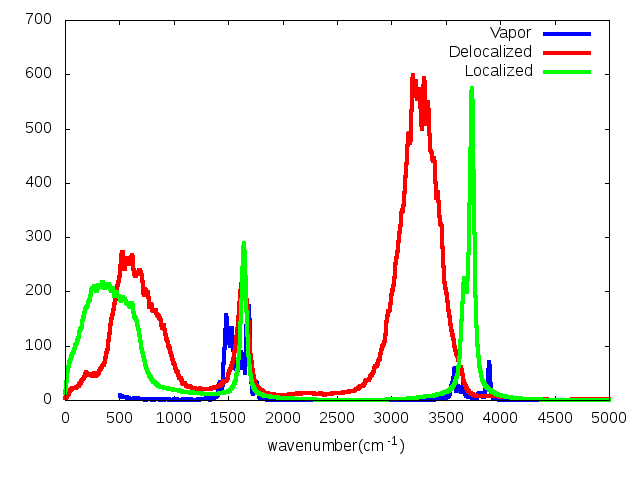
\includegraphics[width=0.4\textwidth]{all_ir}
\caption{IR spectrum. For water vapor, localized and delocalized systems.\new  The low wavenumber part of the spectrum for vapor which corresponds to vibarational modes are not shown for simplicity. \old The O-H stretch mode ($\sim$3600 cm$^{-1}$) for localized system is very similar to vapor which is none-interaction. And the intermolecular modes ($\sim$500 cm$^{-1}$) moves to the left, indicating the intermolecular banding is weaker. } \label{Fig:IR}
\end{figure}

To understand how the directional feature of HBs depends on covalency, we look at the spacial distribution function of Oxygen atom, and the distribution of the H-O-O angle, shown in Fig~\ref{Fig:SDF}. 

\begin{figure}
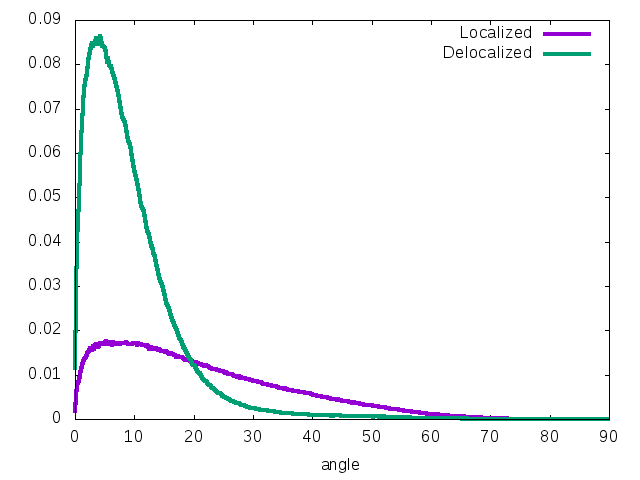
\includegraphics[width=0.225\textwidth]{angular_dist}
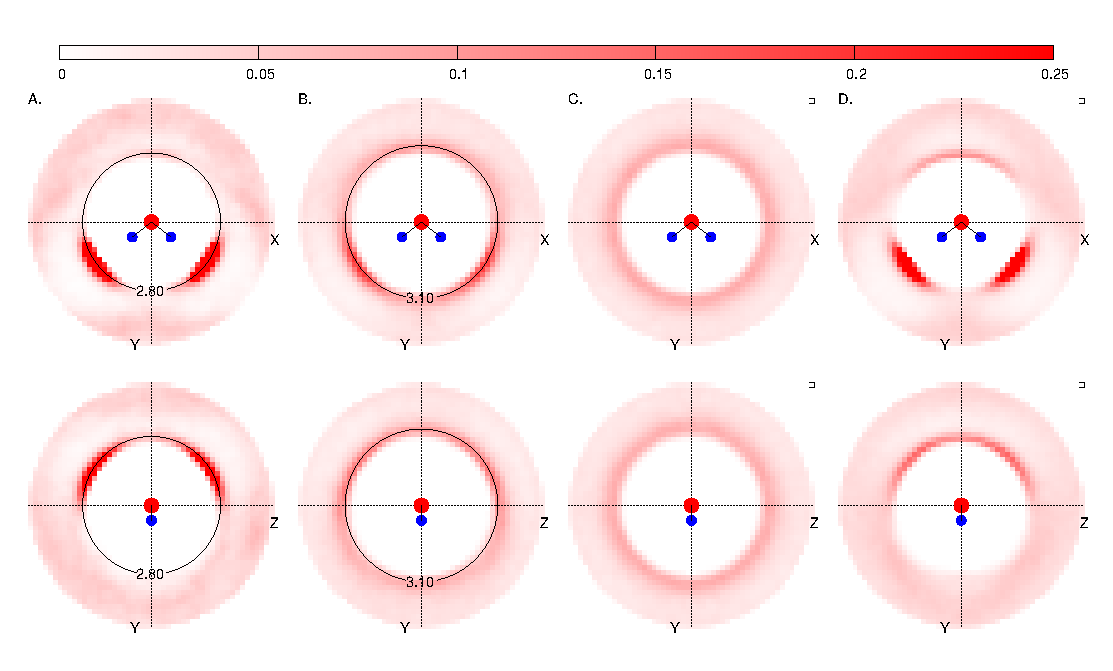
\includegraphics[width=0.225\textwidth]{SDF}
\caption{angular and spacial distribution. } \label{Fig:SDF}
\end{figure}

\textbf{Acknowledgments.} The research was funded by the Natural Sciences and Engineering Research Council of Canada through the Discovery Grant. The authors are grateful to Compute Canada and McGill HPC Centre for computer time.
\bibliography{covalency}
\end{document}
